% Sketch output, version 0.3 (build 2d, Wed Apr 20 23:38:45 2011)
% Output language: PGF/TikZ,LaTeX
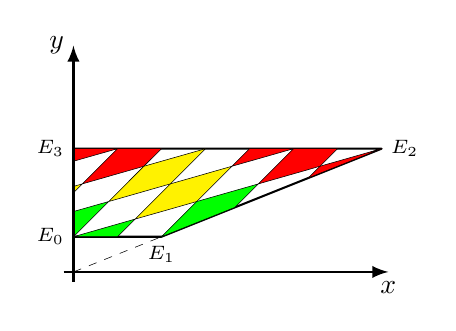
\begin{tikzpicture}[line join=round,line width=0.2pt,>=latex]
\filldraw[fill=none,line width=0.75pt](0,-15.553)--(1.118,-15.553)--(3.913,-14.435)--(0,-14.435)--cycle;
\draw[dashed](0,-16)--(1.118,-15.553);
\filldraw[fill=red](2.981,-14.807)--(3.913,-14.435)--(3.13,-14.658)--cycle;
\filldraw[fill=red](2.348,-14.882)--(3.13,-14.658)--(3.354,-14.435)--(2.795,-14.435)--cycle;
\filldraw[fill=red](2.236,-14.435)--(2.012,-14.658)--(2.795,-14.435)--cycle;
\filldraw[fill=red](.559,-14.435)--(.112,-14.882)--(.894,-14.658)--(1.118,-14.435)--cycle;
\filldraw[fill=red](0,-14.435)--(0,-14.594)--(.559,-14.435)--cycle;
\filldraw[fill=yellow](.783,-15.329)--(1.565,-15.106)--(2.012,-14.658)--(1.23,-14.882)--cycle;
\filldraw[fill=yellow](.894,-14.658)--(.447,-15.106)--(1.23,-14.882)--(1.677,-14.435)--cycle;
\filldraw[fill=yellow](.112,-14.882)--(0,-14.994)--(0,-14.914)--cycle;
\filldraw[fill=green](1.118,-15.553)--(2.05,-15.18)--(2.348,-14.882)--(1.565,-15.106)--cycle;
\filldraw[fill=green](0,-15.553)--(.559,-15.553)--(.783,-15.329)--cycle;
\filldraw[fill=green](0,-15.553)--(.447,-15.106)--(0,-15.233)--cycle;
\draw[->,line width=1pt](0,-16.125)--(0,-13.125);
\draw[->,line width=1pt](-.125,-16)--(4,-16);

    \coordinate [label=below:$x$] (X) at (4,-16);
    \coordinate [label=left:$y$] (Y) at (0,-13.125);
  
    \coordinate [label=180:\scriptsize$E_0$] (p0E) at (0,-15.553);
    \coordinate [label=270:\scriptsize$E_1$] (p1E) at (1.118,-15.553);
    \coordinate [label=000:\scriptsize$E_2$] (p2E) at (3.913,-14.435);
    \coordinate [label=180:\scriptsize$E_3$] (p3E) at (0,-14.435);
  \end{tikzpicture}% End sketch output
